%%% Simon's Workfile! %%%
%%% DESIGN PART %%%

\chapter{Design}
\section{Introduction to design}
As it was earlier decided to create some graphical interface for the game, in form of Unity, some considerations was to be made in regards to the layout. This chapter of the report will focus on the decisions taken, to create a smooth interface and a good user experience. In order to create a smooth interface that would excite people in using the setup at the library, a background, some character and some interaction was to be made. Figure \eqref{fig:ip_Background}
\begin{figure}[htbp]
\centering
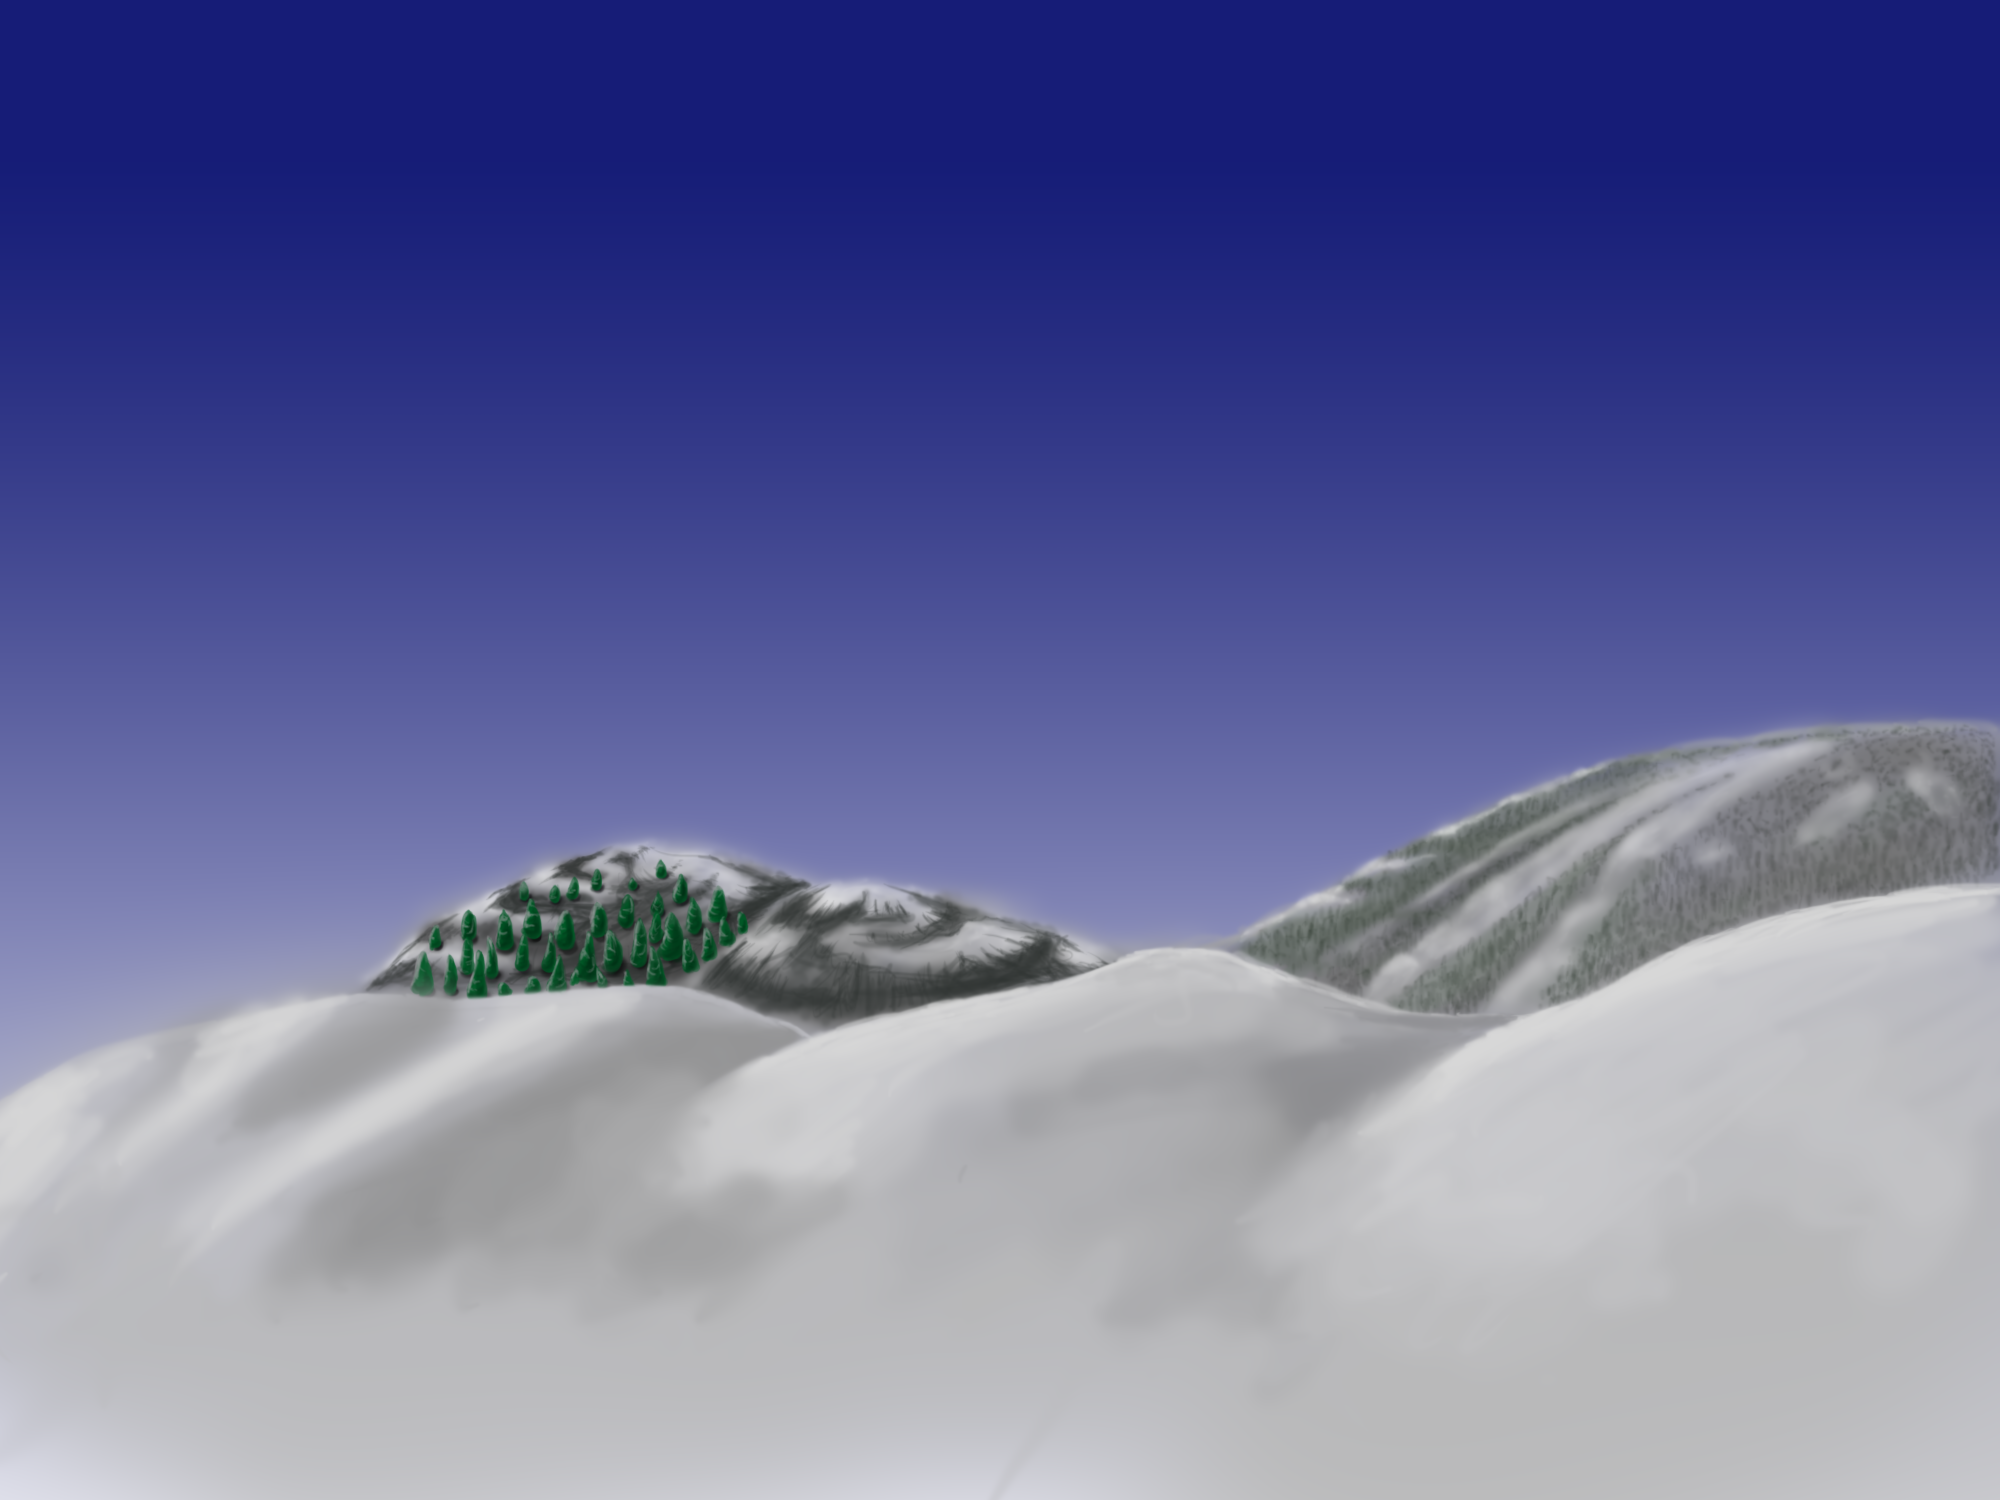
\includegraphics[width=1.00\textwidth]{Pictures/Design/Background.png}
\caption{Image illustrating the initial background for the Christmas game}
\label{fig:ip_Background}
\end{figure}\\ 
\section{The scene}
The first step into developing a good looking set was to develop a suitable background that ultimately would create a Christmas-like mood. The original idea was to have a few different sets to choose from, depending on the time of the day or week. However initially one background was created to run the prototype testing on. The first background created consist of a static winter landscape, together with some dynamic movable trees.\\
In addition; due to light conditions at the library the colors chosen for the background are not all bright, but slightly soften. This action was taken in order for the projector to output a usable illustration.
\section{Avatars}
In addition to the background created for the illustration at the library, some avatars were to be made. Considerations towards creating suitable avatars were made and it was decided to create a pixie boy- and girl, a snowman, an angle and a squirrel.
\subsection{Self-drawn}
In addition it was decided to draw the avatars instead of using some premade drawings on the internet, to be imported as assets in Unity. It was done by drawing the avatars on a sheet of paper and then imported to the computer to be redone in Photoshop with an drawing pen.\\
Considering the primary group of people trespassing the setup at the library, it was decided to give the avatars a cartoonish look. This was done by using a variety of techniques, one of them was to create oversized bodyparts e.g. oversized heads.

\section{Animations}
\subsection{Why animations and which}
\section{Sprite sheets}

